
\section{Model View Controller}

To ensure that code is correctly decoupled from one another, strict
design patterns are necessary, as these allow developing complex projects
without losing sight of the entire project. If no pattern is followed,
code can easily become so entangled that later development might prove
impossible. This section will cover all the rules and ideas behind
the MVC (Model-View-Controller) design pattern. ~\cite{WikiMVC} provides
a short introduction to MVC, although complete comprehension of the
design pattern requires experience using it. Hence, this section will
be based on our prior experiences with MVC.

The MVC pattern principle is that programs that can be interacted
with by a user can be split into three different components. These
components are as follows:
\begin{itemize}
\item Model -- Core of the program
\item View -- Visualization of the program
\item Controller -- Manager of state changes to the core of the program
\end{itemize}
\begin{figure}
\centering{}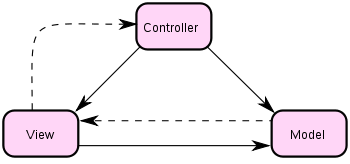
\includegraphics{MVC}\caption{\label{fig:MVCBasic}This image shows how the three components are
connected to each other; the full arrows indicate that a component
has complete knowledge of the component it is pointing to. A dashed
arrow indicates that the component the dashed arrow is pointing to
is listening to the component the arrow is originating from. (Image
taken from \texttt{www.htmlgoodies.com/img/2010/11/mvc.png})}
\end{figure}



\subsection{Model}

The model is the core of the program. It is why the program functions
as it does, it contains all the data, and it is here all business
logic is located. The model should have no knowledge of either the
view or the controller; by not knowing either the program is ensured
to not be tainted by their influence.

While it may not know of the view or the controller, it is paramount
that the model is built to optimally transfer information concerning
its current state. That means that providing a way for other components
to listen on the model is very welcome\emph{. }This gives the model
a way to publish its state when it has been altered\emph{.} What this
does for the model is, that in case the model state has been altered,
it will have a way to provide the information of the state. 

If such features are not built into the model, it would require the
component changing the state to inform of the state changes, in case
of a MVC design. The component changing state is the controller and
as such the controller would have both the duty of changing the state
of the model and maintaining the view. This is generally a case of
a badly designed model and can be completely avoided if the model
simply has the ability to inform its listeners(such as a view) of
any changes.


\subsection{View}

The view is a way to visualize what is currently occurring inside
the model by visualizing it to the user. A view may take many shapes
depending on the model. If, for instance, the model is a program processing
data on a server, then the view could take the form of a logging console.
Or if the model was a computer game then the view would be the graphic
representation of the game. Additionally, a model can have several
views, each displaying information in a different manner. For example,
the computer game mentioned above could also feature a view printing
debugging information to a console while the game was running. Generally,
a view should only have knowledge of the model and not the controller.
The idea is that if the view can see all model data then interaction
with the controller should not be necessary.

When designing a view there are some common pitfalls that can be avoided
with careful design. First off, the view is what it is named: a view.
This means that it should never do any state changes to the model.
If getting hold of data means that the model must change its state
to accommodate this, then the model is poorly made and should be changed.
However, a view is allowed to change its own state without involving
either the controller or model. To fully understand what is meant
by this, consider the following example:

Assume you have a menu bar as depicted in fig. \ref{fig:menubar}.

\begin{figure}[H]
\begin{centering}
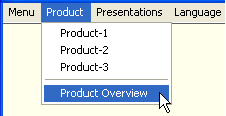
\includegraphics{MenuBar}
\par\end{centering}

\caption{\label{fig:menubar}A standard menu bar.}
\end{figure}


To open a menu, the user need to drag the mouse and click on one menu
he or she wishes to open. Many would see this as a task of the controller.
This is not the case, however, since the changes done are only performed
on the view's own state and not the model of the program.


\subsection{Controller}

The controller is the link between the model and the user. By convention,
all changes the user wishes to perform on the model should be done
through the controller. Like the view, it can take many shapes, like
an object that transforms input from the mouse into changes to the
model, or an object controlling how a network data stream effects
on the model. 

In a well-designed program the controller should never have to interact
with the view. However, this can be practically impossible on larger
projects unless they are carefully planned, and as such the controller
by convention is allowed to know of both the view and the model.

A common mistake when designing the controller is to mistake the unit
which the controller gets input from as the actual controller. In
many cases, the keyboard is the device from which input is transformed
into state changes to the model. However, that does not mean that
the controller should be the only unit interacting with the keyboard.
Going back to the example used to understand the view, the reason
why the controller should not deal with opening a menu bar on the
view is because the controller is not responsible of the state of
the view. The controller is only responsible for the state of the
model; the only case in which it is allowed for the controller to
interfere with the view is in the case that the model was unsuccessful
in properly informing about its state change caused by the controller.
In this case it is okay for the controller to call the view and ask
it to adjust itself. 

The reasoning for why the controller is normally mistaken to be responsible
for handling changes to the state of the view is because it is mistakenly
thought of as a controller for the entire program and not the model,
a view may contain its own controller which should not be mistaken
from the other controller. To fully understand this, imagine that
the view in itself also contains a MVC inside itself (see fig. \ref{fig:MVCeption}).

\begin{figure}[h]
\begin{centering}
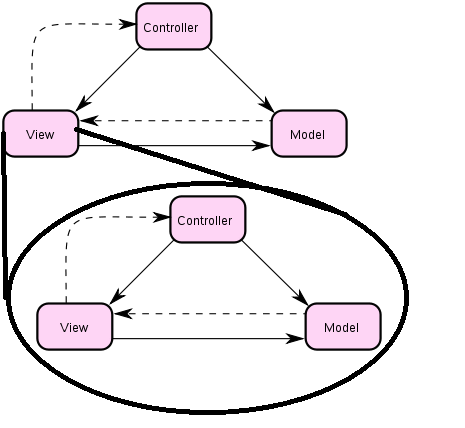
\includegraphics[width=0.6\textwidth]{MVCeption}
\par\end{centering}

\caption{\label{fig:MVCeption}A view with a MVC inside of it.}
\end{figure}


The model of a view (such as a menu bar) would contain data about
the names of the menus and it would be responsible for ordering and
accessing information as to what each menu contains. Its view would
be that of a drawing board responsible for properly drawing the menu
bars. Luckily, most views are simple, so one does not need to make
an entire MVC design, but for graphical user interfaces used in most
operating system it is very important to understand that a view can
be an entire MVC setup in itself. This is why most operating system
comes with libraries to easily design GUI.
